\documentclass[11pt,compress,t,notes=noshow, xcolor=table]{beamer}
\usepackage[]{graphicx}\usepackage[]{color}
% maxwidth is the original width if it is less than linewidth
% otherwise use linewidth (to make sure the graphics do not exceed the margin)
\makeatletter
\def\maxwidth{ %
  \ifdim\Gin@nat@width>\linewidth
    \linewidth
  \else
    \Gin@nat@width
  \fi
}
\makeatother

\newcommand{\citebutton}[2]{%
\beamergotobutton{\href{#2}{#1}}%
}

\newcommand{\blu}[1]{\textcolor{blue}{#1}}
\newcommand{\org}[1]{\textcolor{orange}{#1}}
\newcommand{\ques}{\textbf{\textcolor{red}{Question:  }}}
\newcommand{\questionssofar}{\begin{frame}\frametitle{Any questions?}\end{frame}}

\newcommand\warning{%
 \makebox[1.4em][c]{%
 \makebox[0pt][c]{\raisebox{.1em}{\scriptsize!}}%
 \makebox[0pt][c]{\color{red}\normalsize$\bigtriangleup$}}}%

\definecolor{fgcolor}{rgb}{0.345, 0.345, 0.345}
\newcommand{\hlnum}[1]{\textcolor[rgb]{0.686,0.059,0.569}{#1}}%
\newcommand{\hlstr}[1]{\textcolor[rgb]{0.192,0.494,0.8}{#1}}%
\newcommand{\hlcom}[1]{\textcolor[rgb]{0.678,0.584,0.686}{\textit{#1}}}%
\newcommand{\hlopt}[1]{\textcolor[rgb]{0,0,0}{#1}}%
\newcommand{\hlstd}[1]{\textcolor[rgb]{0.345,0.345,0.345}{#1}}%
\newcommand{\hlkwa}[1]{\textcolor[rgb]{0.161,0.373,0.58}{\textbf{#1}}}%
\newcommand{\hlkwb}[1]{\textcolor[rgb]{0.69,0.353,0.396}{#1}}%
\newcommand{\hlkwc}[1]{\textcolor[rgb]{0.333,0.667,0.333}{#1}}%
\newcommand{\hlkwd}[1]{\textcolor[rgb]{0.737,0.353,0.396}{\textbf{#1}}}%
\let\hlipl\hlkwb

\usepackage{framed}
\makeatletter
\newenvironment{kframe}{%
 \def\at@end@of@kframe{}%
 \ifinner\ifhmode%
  \def\at@end@of@kframe{\end{minipage}}%
  \begin{minipage}{\columnwidth}%
 \fi\fi%
 \def\FrameCommand##1{\hskip\@totalleftmargin \hskip-\fboxsep
 \colorbox{shadecolor}{##1}\hskip-\fboxsep
     % There is no \\@totalrightmargin, so:
     \hskip-\linewidth \hskip-\@totalleftmargin \hskip\columnwidth}%
 \MakeFramed {\advance\hsize-\width
   \@totalleftmargin\z@ \linewidth\hsize
   \@setminipage}}%
 {\par\unskip\endMakeFramed%
 \at@end@of@kframe}
\makeatother

\definecolor{shadecolor}{rgb}{.97, .97, .97}
\definecolor{messagecolor}{rgb}{0, 0, 0}
\definecolor{warningcolor}{rgb}{1, 0, 1}
\definecolor{errorcolor}{rgb}{1, 0, 0}
\newenvironment{knitrout}{}{} % an empty environment to be redefined in TeX

\usepackage{alltt}
\newcommand{\SweaveOpts}[1]{}  % do not interfere with LaTeX
\newcommand{\SweaveInput}[1]{} % because they are not real TeX commands
\newcommand{\Sexpr}[1]{}       % will only be parsed by R
\newcommand{\xmark}{\ding{55}}%


\usepackage[english]{babel}
\usepackage[utf8]{inputenc}

\usepackage{dsfont}
\usepackage{verbatim}
\usepackage{amsmath}
\usepackage{amsfonts}
\usepackage{amssymb}
\usepackage{bm}
\usepackage{csquotes}
\usepackage{multirow}
\usepackage{longtable}
\usepackage{booktabs}
\usepackage{enumerate}
\usepackage[absolute,overlay]{textpos}
\usepackage{psfrag}
\usepackage{algorithm}
\usepackage{algpseudocode}
\usepackage{eqnarray}
\usepackage{arydshln}
\usepackage{tabularx}
\usepackage{placeins}
\usepackage{tikz}
\usepackage{setspace}
\usepackage{colortbl}
\usepackage{mathtools}
\usepackage{wrapfig}
\usepackage{bm}
\usepackage{amsmath}
\usepackage{pifont}

\usetikzlibrary{shapes.multipart,shapes,arrows,automata,positioning,calc,chains,trees, shadows}
\tikzset{
  %Define standard arrow tip
  >=stealth',
  %Define style for boxes
  punkt/.style={
    rectangle,
    rounded corners,
    draw=black, very thick,
    text width=6.5em,
    minimum height=2em,
    text centered},
  % Define arrow style
  pil/.style={
    ->,
    thick,
    shorten <=2pt,
    shorten >=2pt,}
}

\tikzstyle{vec}=[draw, rectangle, fill = white, minimum width=5mm, minimum height=1cm, inner sep = 2pt]

\usepackage{subfig}

% Defines macros and environments
\usepackage{../../style/lmu-lecture}


\let\code=\texttt
\let\proglang=\textsf

\setkeys{Gin}{width=0.9\textwidth}

\setbeamertemplate{frametitle}{\expandafter\uppercase\expandafter\insertframetitle}

\usepackage{bbm}
% basic latex stuff
\newcommand{\pkg}[1]{{\fontseries{b}\selectfont #1}} %fontstyle for R packages
\newcommand{\lz}{\vspace{0.5cm}} %vertical space
\newcommand{\dlz}{\vspace{1cm}} %double vertical space
\newcommand{\oneliner}[1] % Oneliner for important statements
{\begin{block}{}\begin{center}\begin{Large}#1\end{Large}\end{center}\end{block}}


%new environments
\newenvironment{vbframe}  %frame with breaks and verbatim
{
 \begin{frame}[containsverbatim,allowframebreaks]
}
{
\end{frame}
}

\newenvironment{vframe}  %frame with verbatim without breaks (to avoid numbering one slided frames)
{
 \begin{frame}[containsverbatim]
}
{
\end{frame}
}

\newenvironment{blocki}[1]   % itemize block
{
 \begin{block}{#1}\begin{itemize}
}
{
\end{itemize}\end{block}
}

\newenvironment{fragileframe}[2]{  %fragile frame with framebreaks
\begin{frame}[allowframebreaks, fragile, environment = fragileframe]
\frametitle{#1}
#2}
{\end{frame}}


\newcommand{\myframe}[2]{  %short for frame with framebreaks
\begin{frame}[allowframebreaks]
\frametitle{#1}
#2
\end{frame}}

\newcommand{\remark}[1]{
  \textbf{Remark:} #1
}


\newenvironment{deleteframe}
{
\begingroup
\usebackgroundtemplate{
\includegraphics[width=\paperwidth,height=\paperheight]{../style/color/red.png}}
 \begin{frame}
}
{
\end{frame}
\endgroup
}
\newenvironment{simplifyframe}
{
\begingroup
\usebackgroundtemplate{
\includegraphics[width=\paperwidth,height=\paperheight]{../style/color/yellow.png}}
 \begin{frame}
}
{
\end{frame}
\endgroup
}\newenvironment{draftframe}
{
\begingroup
\usebackgroundtemplate{
\includegraphics[width=\paperwidth,height=\paperheight]{../style/color/green.jpg}}
 \begin{frame}
}
{
\end{frame}
\endgroup
}
% https://tex.stackexchange.com/a/261480: textcolor that works in mathmode
\makeatletter
\renewcommand*{\@textcolor}[3]{%
  \protect\leavevmode
  \begingroup
    \color#1{#2}#3%
  \endgroup
}
\makeatother





\input{../../latex-math/basic-math.tex}
\input{../../latex-math/basic-ml.tex}

%\newcommand{\titlefigure}{figure/gpt_sq.png}
\newcommand{\learninggoals}{
\item Recall the concept of optimization
\item Understand basics of gradient descent}

\title{Deep Learning basics}
% \author{}
\institute{\href{https://slds-lmu.github.io/lecture_dl4nlp/}{slds-lmu.github.io/lecture\_dl4nlp}}
\date{}

\begin{document}
\lecturechapter{Optimization and Gradient Descent}
\lecture{Deep Learning for NLP}

% ------------------------------------------------------------------------------

\begin{vbframe}{Optimization}

\vfill

\begin{itemize}
\item Optimization: Minimize some function $J(\vec \theta)$ by altering $\vec \theta$.
\item Maximize $f(\vec \theta)$ by minimizing $J(\vec \theta) = - f(\vec \theta)$
\item $J(\vec \theta)$:
\begin{itemize}
 \item \emph{``criterion'', ``objective function'', ``cost function'', ``loss function'', ``error function''}
 \item In a probabilistic machine learning setting often (conditional) negative log-likelihood:
 $$- \log p(\vec X; \vec \theta)$$
 or
 $$- \log p(\vec y|\vec X; \vec \theta)$$
 as a function of $\vec \theta$
\item $\vec \theta^* = \arg\min_{\vec\theta} J(\vec \theta)$

\end{itemize}
\end{itemize}
\begin{center}
%\includegraphics[width = 0.5\textwidth]{./}
\end{center}

\vfill

\end{vbframe}


% ------------------------------------------------------------------------------

\begin{vbframe}{Optimization}

\vfill

%DL Ch. 4.3
\begin{itemize}
\item If $J(\vec \theta)$ is convex, it is minimized where $\nabla_{\vec\theta} J(\vec \theta) = \vec 0$
\item If $J(\vec \theta)$ is not convex, the gradient can help us to improve our objective nevertheless (and find a local optimum).
\item Many optimization techniques were originally developed for convex objective functions, but are found to be working well for non-convex functions too.
\item Use the fact that gradient indicates the slope of the function in the direction of steepest increase.
\begin{center}
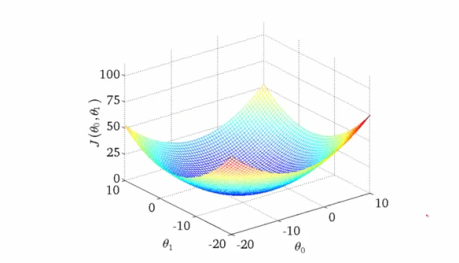
\includegraphics[width = 0.49\textwidth]{./figure/convex_cost_function} 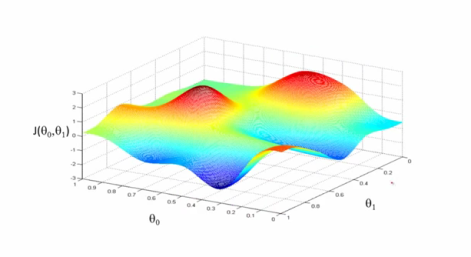
\includegraphics[width = 0.49\textwidth]{./figure/nonconvex}
\end{center}

\end{itemize}
\begin{center}
%\includegraphics[width = 0.5\textwidth]{./}
\end{center}

\vfill

\end{vbframe}


% ------------------------------------------------------------------------------

\begin{vbframe}{Gradient-Based Optimization}

\vfill

\begin{itemize}
\item Derivative: Given a small change in input, what is the corresponding change in output?
$$f(x + \epsilon) \approx f(x) + \epsilon f'(x) $$
\begin{center}
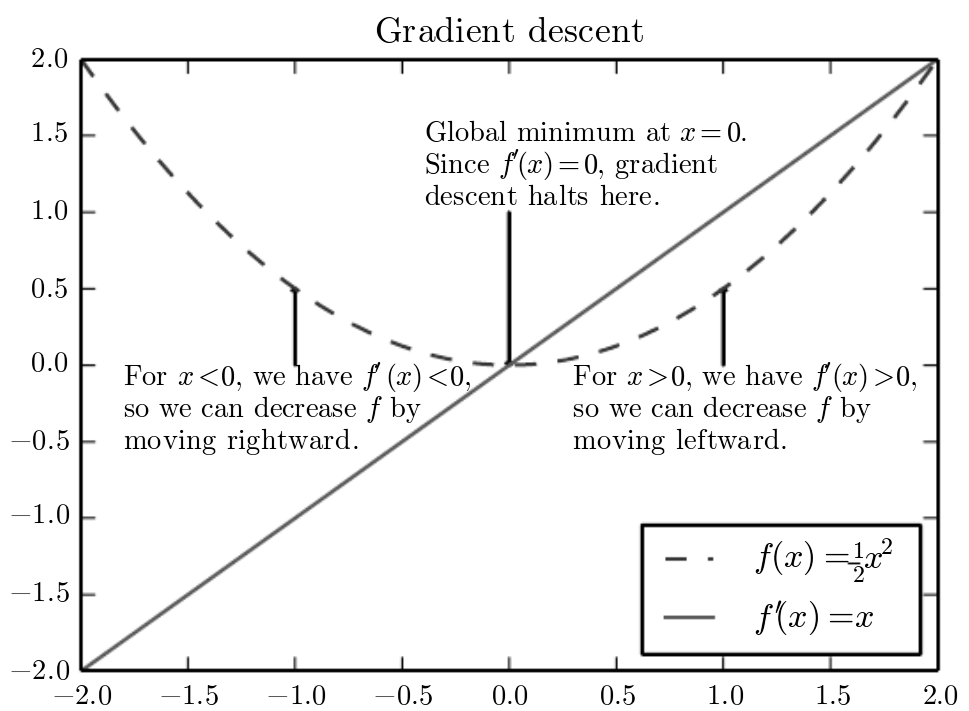
\includegraphics[width = 0.5\textwidth]{./figure/gradient_descent}
\end{center}
\item $f(x - \epsilon \sign f'(x)) < f(x)$ for small enough $\epsilon$
\end{itemize}

\vfill

\end{vbframe}


% ------------------------------------------------------------------------------

\begin{vbframe}{Gradient Descent}

\vfill

\begin{itemize}
\item For $J(\vec \theta): \mathbb{R}^n \to \mathbb{R}$\\
\item If partial derivative $\frac{\partial J(\vec \theta)}{\partial \theta_j} > 0$, $J(\vec \theta)$ will increase for small increases of $\theta_j$\\
$\Rightarrow$ go in opposite direction of gradient (since we want to minimize)
\item Steepest descent: iterate
$$\vec \theta_{t+1} \leftarrow \vec \theta_t - \eta \nabla_{\vec \theta} J(\vec \theta_t)$$
where $\vec\theta_t$ is the actual parameter, $J(\vec \theta_t)$ is the objective function evaluated at $\vec\theta_t$
and $\vec\theta_{t+1}$ is the updated parameter.
\item $\eta$ is the learning rate (set to small positive constant).
\item Converges if $\nabla_{\vec \theta} J(\vec \theta)$ is (close to) $\vec 0$
%\item Simple function can sometimes directly be solved for $\nabla_{\vec \theta} J(\vec \theta) = \vec 0$
\end{itemize}

\vfill

\end{vbframe}


% ------------------------------------------------------------------------------

\begin{vbframe}{Local Minima}

\vfill

\begin{itemize}
\item If the function is non-convex, different results can be obtained at convergence, depending on initialization of $\vec \theta$.
\end{itemize}
\begin{center}
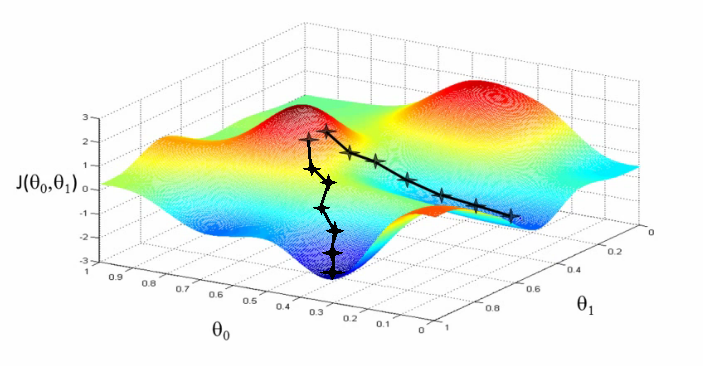
\includegraphics[width = 0.8\textwidth]{./figure/gradient-descent}
\end{center}

\vfill

\end{vbframe}


% ------------------------------------------------------------------------------

\begin{vbframe}{Local Minima}

\vfill

\begin{itemize}
\item Minima can be global or local:
\begin{center}
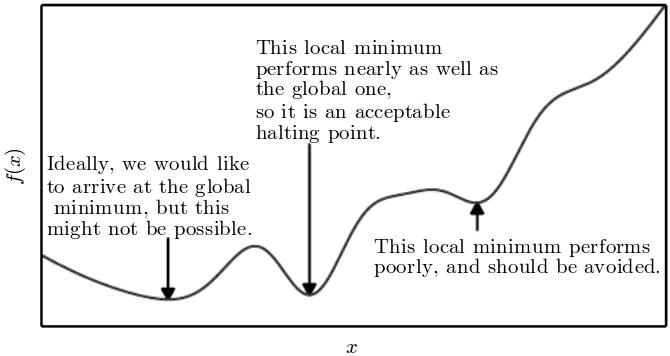
\includegraphics[width = 0.6\textwidth]{./figure/local_minima}
\end{center}
\item Critical (stationary) points:  $f'(x) = 0$
\begin{center}
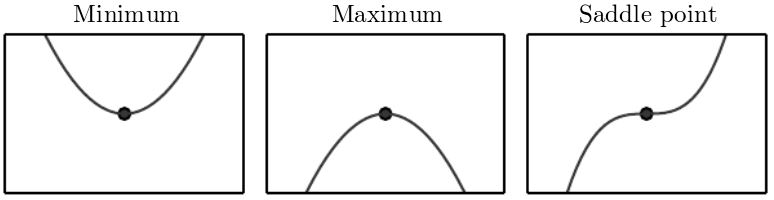
\includegraphics[width = 0.5\textwidth]{./figure/critical_points}
\end{center}
\item For neural networks, only good (not perfect) parameter values can be found.
\end{itemize}

\vfill

\end{vbframe}


% ------------------------------------------------------------------------------

\begin{vbframe}{Gradient Descent for Logistic Regression}

\vfill

$$\nabla_{\vec\theta} NLL(\vec \theta) =  -\nabla_{\vec\theta} \sum_{i=1}^m y^{(i)} \log \sigma(\vec{\theta}^T \vec{x^{(i)}}) + (1-y^{(i)}) \log (1 - \sigma(\vec{\theta}^T \vec{x^{(i)}}))$$
$$= - \sum_{i=1}^m (y^{(i)} - \sigma(\vec{\theta}^T \vec{x^{(i)}})) \vec{x^{(i)}}  $$
\begin{itemize}
\item The gradient descent update becomes:
$$\vec{\theta}_{t+1} := \vec{\theta}_{t} + \eta \sum_{i=1}^m (y^{(i)} - \sigma(\vec{\theta}_{t}^T \vec{x}^{(i)})) \vec{x}^{(i)} $$

\item Note: Which feature weights are increased, which are decreased?
\end{itemize}
\begin{center}
%\includegraphics[width = 0.5\textwidth]{./}
\end{center}

\vfill

\end{vbframe}


% ------------------------------------------------------------------------------

\begin{vbframe}{Derivation of Gradient for Logistic Regression}

\vfill

This is a great exercise! Use the following facts:\\
\vspace{.2cm}
\renewcommand{\arraystretch}{2}
\begin{tabular}{r|l}
Gradient & $(\nabla_{\vec\theta} f(\vec \theta))_j = \frac{\partial f(\vec \theta)}{\partial \theta_j}$\\
%\hline
Derivative of a sum & $\frac{d}{dz}\sum_i f_i(z) = \sum_i \frac{df_i(z)}{dz} $\\

Chain rule & $F(z) = f(g(z))$ \ $\Rightarrow$ \ $F'(z) = f'(g(z)) g'(z)$\\
Derivative of logarithm & $\frac{d \log z}{dz} = 1/z$\\
D. of logistic sigmoid & $\frac{d \sigma(z)}{dz} = \sigma(z)(1-\sigma(z))$\\
Partial d. of dot-product & $\frac{\partial \vec{\theta}^T \vec x}{\partial \theta_j} = \vec{x}_j$\\
\end{tabular}
%
%\begin{itemize}
%\end{itemize}

\vfill

\end{vbframe}


% ------------------------------------------------------------------------------

\begin{vbframe}{Gradient Descent: Summary}

\vfill

\begin{itemize}
\item Iterative method for function minimization.
\item Gradient indicates rate of change in objective function, given a local change to feature weights.
\item Substract the gradient: 
\begin{itemize}
 \item \textbf{decrease} parameters that (locally) have \textbf{positive} correlation with objective
 \item \textbf{increase} parameters that (locally) have \textbf{negative} correlation with objective
\end{itemize}
\item Gradient updates only have the desired properties in a small region around previous parameters $\vec \theta_t$. Control locality by step-size $\eta$.
\item Gradient descent is slow: For relatively small step in the right direction, all of training data has to be processed.
\item This version of gradient descent is often also called \emph{batch gradient descent}.
\end{itemize}

\vfill

\end{vbframe}


% ------------------------------------------------------------------------------

\begin{vbframe}{Stochastic Gradient Descent (SGD)}

\vfill

\begin{itemize}
\item \emph{Batch gradient descent} is slow: For relatively small step in the right direction, all of training data has to be processed.

%$$\vec g = - \nabla_{\theta} \sum_{i=1}^m \log  p(y_i | \vec x_i; \vec \theta)$$
%$$\vec \theta_{t+1} \leftarrow \vec \theta_t - \eta \vec g$$

$$\vec \theta_{t+1} \leftarrow \vec \theta_t + \eta \nabla_{\vec\theta} \sum_{i=1}^m \log  p(y_i | \vec x_i; \vec \theta)$$


\item \emph{Stochastic gradient descent} in a nutshell:
\begin{itemize}
 \item For each update, only use random sample $\mathbb{B}_t$ of training data (mini-batch).

$$\vec \theta_{t+1} \leftarrow \vec \theta_t + \eta \nabla_{\vec\theta} \sum_{i \in \mathbb{B}_t} \log  p(y_i | \vec x_i; \vec \theta)$$

%$$\vec g = - \frac{1}{|\mathbb{B}_t|} \nabla_{\theta} \sum_{i \in \mathbb{B}_t} \log  p(y_i | \vec x_i; \vec \theta)$$ 
 
 \item Mini-batch size can also just be $1$.
$$\vec \theta_{t+1} \leftarrow \vec \theta_t + \eta \nabla_{\vec\theta} \log  p(y_t | \vec x_t; \vec \theta)$$ 
% $$\vec{\theta}_{t+1} \leftarrow \vec{\theta}_{t} + \eta (y^{(i)} - \sigma(\vec{\theta}_{t}^T \vec{x}^{(i)})) \vec{x}^{(i)} $$
\end{itemize}
\item $\Rightarrow$ More frequent updates.
\end{itemize}

\vfill

\end{vbframe}


% ------------------------------------------------------------------------------

\begin{vbframe}{Stochastic Gradient Descent (SGD)}

\vfill

\begin{itemize}
\item The actual gradient is \emph{approximated} using only a sub-sample of the data.
\item For objective functions that are highly non-convex, the random deviations of these approximations may even help to escape local minima.
\item Treat batch size and learning rate as hyper-parameters.
\end{itemize}
\begin{center}
%\includegraphics[width = 0.5\textwidth]{./}
\end{center}

\vfill

\end{vbframe}



\endlecture
\end{document}
